\documentclass[tikz,border=9pt]{standalone}
\usepackage[utf8]{inputenc}
\usepackage[OT4,plmath]{polski}
\usepackage{amsmath}
\begin{document}
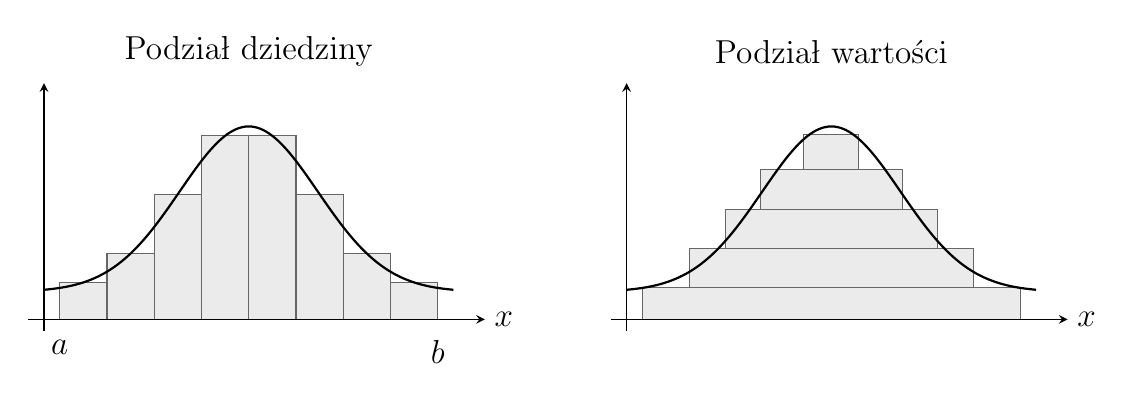
\begin{tikzpicture}[font=\large,>=stealth]
  \begin{scope}
    \node at (2.6,3.4) {Podział dziedziny};
    \foreach \i in {0,...,7} {
      \pgfmathsetmacro{\lft}{0.2+0.6*\i}
      \pgfmathsetmacro{\rgt}{\lft+0.6}
      \pgfmathsetmacro{\midp}{\lft+0.3}
      \pgfmathsetmacro{\htval}{0.35+2.1*exp(-0.65*(\midp-2.6)^2)}
      \filldraw[fill=black!8,draw=black!60] (\lft,0) rectangle (\rgt,\htval);
    }
    \draw[thick,domain=0:5.2,samples=70,smooth]
      plot (\x,{0.35+2.1*exp(-0.65*(\x-2.6)^2)});
    \draw[->] (-0.2,0)--(5.6,0) node[right] {$x$};
    \draw[->] (0,-0.15)--(0,3.0);
    \node[below=4pt] at (0.2,0) {$a$};
    \node[below=4pt] at (5,0) {$b$};
  \end{scope}
  \begin{scope}[xshift=7.4cm]
    \node at (2.6,3.4) {Podział wartości};
    \foreach \left/\right/\low/\high in {
      0.2/5.0/0/0.4,
      0.8/4.4/0.4/0.9,
      1.25/3.95/0.9/1.4,
      1.7/3.5/1.4/1.9,
      2.25/2.95/1.9/2.35} {
      \filldraw[fill=black!8,draw=black!60] (\left,\low) rectangle (\right,\high);
    }
    \draw[thick,domain=0:5.2,samples=70,smooth]
      plot (\x,{0.35+2.1*exp(-0.65*(\x-2.6)^2)});
    \draw[->] (-0.2,0)--(5.6,0) node[right] {$x$};
    \draw[->] (0,-0.15)--(0,3.0);
  \end{scope}
\end{tikzpicture}
\end{document}
